\documentclass[xcolor={dvipsnames}]{beamer}

\usefonttheme{professionalfonts}
%\usefonttheme{serif}
\usepackage[cochineal]{rntzfont} % pt, charter work well
%\usepackage{PTSans}
\usepackage[semibold]{sourcesanspro}

%\usepackage{booktabs}
\usepackage{anyfontsize} % fix font warnings from stmaryrd
\usepackage{latexsym,amssymb,stmaryrd,mathtools}
\usepackage{mathpartir}
\usepackage{multirow}
\usepackage{tikz,tikz-cd}       % Hasse & commutative diagrams.
\usepackage{url,hyperref}
\usepackage{nccmath}

\usepackage[normalem]{ulem}               % for \sout
\newcommand{\msout}[1]{\text{\sout{\ensuremath{#1}}}}

\definecolor[named]{ACMBlue}{cmyk}{1,0.1,0,0.1}
\definecolor[named]{ACMYellow}{cmyk}{0,0.16,1,0}
\definecolor[named]{ACMOrange}{cmyk}{0,0.42,1,0.01}
\definecolor[named]{ACMRed}{cmyk}{0,0.90,0.86,0}
\definecolor[named]{ACMLightBlue}{cmyk}{0.49,0.01,0,0}
\definecolor[named]{ACMGreen}{cmyk}{0.20,0,1,0.19}
\definecolor[named]{ACMPurple}{cmyk}{0.55,1,0,0.15}
\definecolor[named]{ACMDarkBlue}{cmyk}{1,0.58,0,0.21}

\title{A type system for monotonicity}
\author{Michael Arntzenius}
\institute{University of Birmingham}
\date{ICFP 2018}


%% ===== Commands =====
\newcommand{\R}{\mathbb{R}}
\newcommand{\N}{\mathbb{N}}
\newcommand{\x}{\times}
\newcommand{\G}{\Gamma}
\newcommand{\fn}{\lambda}
\newcommand{\binder}{.~}
\newcommand{\bind}[1]{{#1}\binder}
\newcommand{\fnof}[1]{\fn\bind{#1}}
\newcommand{\den}[1]{\llbracket{#1}\rrbracket}
\newcommand{\bnfeq}{\dblcolon=}
\newcommand{\hilit}{\color{Rhodamine}}
\newcommand{\hil}[1]{{\hilit#1}}

\newcommand{\rulename}{\sffamily\scshape}

\newcommand\opcolor{\color{ForestGreen}}
\newcommand\isocolor{\color{NavyBlue}}
\newcommand\pathcolor{\color{Bittersweet}}

\newcommand{\id}{\text{id}}
\newcommand{\op}{{\text{\opcolor op}}}
\newcommand{\iso}{\ensuremath{{\isocolor\Box}}}
\renewcommand{\path}{\ensuremath{{\pathcolor\lozenge}}}

\newcommand{\idof}{\mathop{\id}}
\newcommand{\opof}{\mathop{\op}}
\newcommand{\isof}{\iso}
\newcommand{\pathof}{\path}

\newcommand\subtype{\mathrel{<:}}
\newcommand\fname[1]{\ensuremath{\mathrm{#1}}}
\newcommand\kw[1]{\mathbf{#1}}
\newcommand\isovar[1]{{#1}}


\begin{document}
\maketitle
\Large

\begin{frame}{}
  It's just the simply-typed $\lambda$-calculus!
  \[\begin{array}{rcll}
    \den{A} &\in& \mathbf{Poset}\vspace{.2em}\\
    {\den{A \to B}}
    &=& \text{\emph{monotone} maps}~ \den{A} \to \den{B},\\
    && \text{ordered pointwise}
  \end{array}\]
\end{frame}

\begin{frame}
  \vspace{-2em}
  \begin{mathpar}
    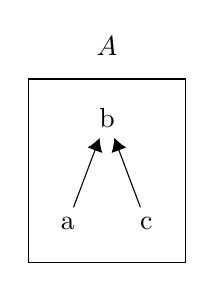
\begin{tikzpicture}[baseline=(current bounding box.center)]
      \node (a) at (-0.5, 0) {a};
      \node (b) at (0, 1.33) {b};
      \node (c) at (.5, 0) {c};
      %% bounding box
      \node [above] at (0, 2) {$A$};
      \draw (-1, 1.83) -- (1, 1.83) -- (1, -0.5) -- (-1, -0.5) -- cycle;
      %% arrows
      \draw [-{Latex[width=2mm]}] (a) -- (b);
      \draw [-{Latex[width=2mm]}] (c) -- (b);
    \end{tikzpicture}

    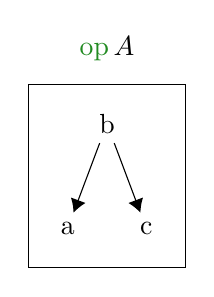
\begin{tikzpicture}[baseline=(current bounding box.center)]
      \node (a) at (-0.5, 0) {a};
      \node (b) at (0, 1.33) {b};
      \node (c) at (.5, 0) {c};
      %% bounding box
      \node [above] at (0, 2) {$\opof A$};
      \draw (-1, 1.83) -- (1, 1.83) -- (1, -0.5) -- (-1, -0.5) -- cycle;
      %% arrows
      \draw [{Latex[width=2mm]}-] (a) -- (b);
      \draw [{Latex[width=2mm]}-] (c) -- (b);
    \end{tikzpicture}

    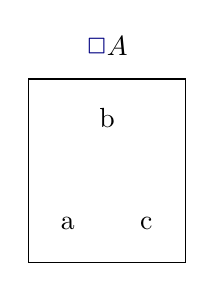
\begin{tikzpicture}[baseline=(current bounding box.center)]
      \node (a) at (-0.5, 0) {a};
      \node (b) at (0, 1.33) {b};
      \node (c) at (.5, 0) {c};
      %% bounding box
      \node [above] at (0, 2) {$\isof A$};
      \draw (-1, 1.83) -- (1, 1.83) -- (1, -0.5) -- (-1, -0.5) -- cycle;
    \end{tikzpicture}
  \end{mathpar}
  \vspace{1em}

  %\pause
  $f : \isof A \to B$ is monotone iff
  \begin{center}
    $x = y \implies f(x) \le f(y)$
  \end{center}
  i.e. \textbf{always}!
\end{frame}

\begin{frame}
  \[\begin{array}{l}
  \fname{setMap} ~:~
  \iso(\iso A \to B) \to \fname{Set}~A \to \fname{Set}~B\\
  \fname{setMap}~f~xs =\\
  \alt<2>{}{\quad\kw{let}~\kw{box}~\isovar{g} = f ~\kw{in}}{}\\
  \quad\kw{do}~x \leftarrow xs\\
  \alt<2>{}{\quad\phantom{\kw{do}~}\kw{let}~\kw{box}~\isovar{y} = x}\\
  \quad\phantom{\kw{do}~}
  \fname{return}~
  \uncover<1>{(\kw{box}~}
  (\alt<2>{f\hspace{2.1pt}}{g}~
  \uncover<1>{(\kw{box}~}\alt<1>{\isovar{y}}{x})\uncover<1>{))}
  \end{array}\]
\end{frame}

\begin{frame}
  \Huge
  \begin{mathpar}
    \uncover<2>{[T]}{} A \subtype B
    \\
    \fname{id} : \uncover<2>{T}{}A \to B
    \\\pause
    T \in \{\id,\op,\iso,...\}
  \end{mathpar}
\end{frame}

\begin{frame}
  \huge
  \begin{mathpar}
    f : TA \to B

    g : UB \to C
    \\
    g \circ f : (UT) A \to C
  \end{mathpar}
\end{frame}

\begin{frame}
  \textbf{Monotonicity tames dragons!}
  \begin{enumerate}
  \item \hil{Eventual consistency} in \hil{distributed systems}\\
    {\small\url{http://bloom-lang.net/calm/}\par}

  \item \Large\hil{Determinism} in \hil{parallel programs}\\
    {\small\emph{LVars: Lattice-based Data Structures for Deterministic
        Parallelism}, Lindsey Kuper \& Ryan Newton\par}
    
  \item \Large\hil{Recursive queries} in \hil{Datalog \& Datafun}\\
    {\small\url{http://www.rntz.net/datafun}\par}

  \item \hil{Paradoxes of self-reference}
  \end{enumerate}
\end{frame}

\begin{frame}
  \Huge\centering\scshape fin
\end{frame}


\newcommand\Z{\mathbb{Z}}

\begin{frame}
  \[\begin{array}{l}
    \fname{subtractEach} ~:~ \fname{List}~(\Z \x \opof\Z) \to \fname{List}~\Z
    \\
    \fname{subtractEach}~xs = [x-y ~|~ (x,y) \leftarrow xs]
  \end{array}\]
\end{frame}

\begin{frame}
  \large
  \begin{mathpar}
    \begin{array}{llc}
      a \le b : \idof A &\iff& a \le b : A\\
      a \le b : \opof A &\iff& a \ge b : A\\
      a \le b : \isof A &\iff& a \le b \wedge a \ge b : A\\
      a \le b : \pathof A &\impliedby& a \le b \vee b \le a : A
    \end{array}

    \begin{tikzpicture}[baseline=(current bounding box.center)]
      \node (top)  at ( 0, 1) {$\path$};
      \node (bot)  at ( 0,-1) {$\iso$};
      \node (-1)   at (-1, 0) {$\id$};
      \node (1)    at ( 1, 0) {$\op$};
      \draw (top) -- (-1) -- (bot) -- (1) -- (top);
    \end{tikzpicture}

    \begin{array}{cr|cccc}
      \multicolumn{2}{c|}{\multirow{2}{*}{$UT$}}
      & \multicolumn{4}{c}{T}\\
      && \id & \op & \iso & \path\\\hline
      \multirow{4}{*}{$U$}
      & \id & \id & \op & \iso & \path\\
      & \op & \op & \id & \iso & \path\\
      & \iso & \iso & \iso & \iso & \path\\
      & \path & \path & \path & \iso & \path
    \end{array}
  \end{mathpar}
\end{frame}

\begin{frame}
  \[
    \infer[\Large subsumption]
          {\G \vdash M : A \\ [T]A \subtype B}
          {T\G \vdash M : C}
  \]
\end{frame}


%% TODO
%% subsumption rule

\end{document}
